\subsection{Towards Realization of Dataspaces}

In the paper ``Towards Realization of Dataspaces'', written by Ibrahim Elsayed and Peter Brezany\cite{1698348}, the architecture and functionality of a Dataspace Management System(DMS) is presented. Additionally it is discussed, how grid technology of future implementations is able to support such an architecture. A DMS is a set of software programs, which controls the organization, storage and retrieval of data in a Dataspace. It also handles the security and integrity of a Dataspace.
In the following, the architecture and the functionality requirements of a DMS will be described.   

\textbf{{\large Requirements}}

\begin{figure}[H]
	\begin{center}
		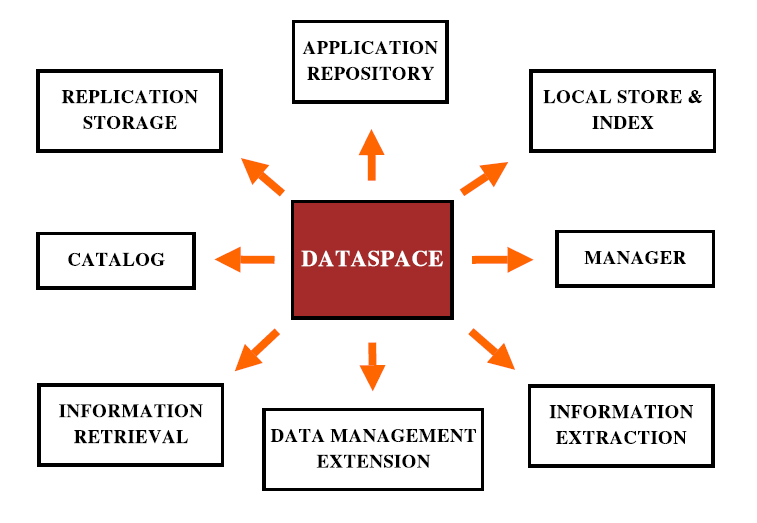
\includegraphics[width=0.75\textwidth]{figures/TowardsRealizationOfDataspaces1.png}
	\end{center}
	\caption{Environment of  a Dataspace}
	\label{TowardsRealizationOfDataspacesEnvironment}
\end{figure}

\uline{Information Retrieval:} Queries and searches are two different methods of information retrieval and represent together one of the main services a DMS should support. Generally, queries and searches should be supported by all participants of the Dataspace, regardless of their used data model. It shouldn't make a difference for a user to operate on a sole database or on a Dataspace. A good known and simple search operation is keyword searching. The Support of spanning such a search method over all participants, is a challenging research topic. The development of methods for keyword searching on relational and XML databases was done by the data-engineering community \cite{994693, Guo:2003:XRK:872757.872762, Hristidis:2002:DKS:1287369.1287427}, For supporting a global query functionality allowing to formulate uniform queries on all Dataspace participants, intelligent methods for interpreting and translating of queries in several languages are required. Methods for query translation were investigated by a large body of research communities \cite{Carey00xperanto:publishing, 1319983}. 

\uline{Information Extraction:} The world-wide web has become a large data container, by now. For allowing to postprocess data obtained from the web, techniques for web information extraction, extracting relevant information from semi-structured web pages should be supported. For further processing, extracted content has to be converted to structured data and saved locally. Non structured web documents have to be classified first using text mining techniques, which organize the parsed documents into groups with the help of ontologies \cite{conf/wise/HeQZW04}. Based on these ontologies, a keyword search is possible to find individual documents. Structured documents allow easier access and integration due to the rich semantically information included in the data representation.\\
\uline{Data Management Extensions:} This component provides possibilities to improve low-level working Dataspace components. All these base components have only limited data management capabilities. It is a task of a DMS to provide additional functionality such as backup, recovery and replication.\\
\uline{Catalog:} Contains a detailed description of all participants of the Dataspace. Beside basic information about the participants, such as owner, creation date, etc., the description for each participant should also contain semantic information about its data. A user should be able to browse the catalog for getting more detailed information about certain data sources. The catalog may reference a meta-data repository to separate the basic and more detailed descriptions.\\
\uline{Manager:} In order to realize the above mentioned functionality, a central component managing the system and interacting with the user is needed. Alongside user authentication, right assignments and other services, this manager component is responsible for communicating with all participants. Thus, this component serves as an interface between the users and the participants of the Dataspace.\\
\uline{Local Store and Index:} This component is responsible for caching search and query results, so that certain queries can be answered without the need of accessing the actual data sources. Furthermore it supports the creation of queryable associations between the participants.\\
\uline{Replication Storage:} Allows to copy participant data in order to increase its access time. This results in high availability and high recovery is supported.\\
\uline{Application Repository:} With this component, the user is able to share data analysis tools, domain specific models, evaluations, etc., which can be applied to the (available) data of the Dataspace.\\
\begin{figure}[H]
	\begin{center}
		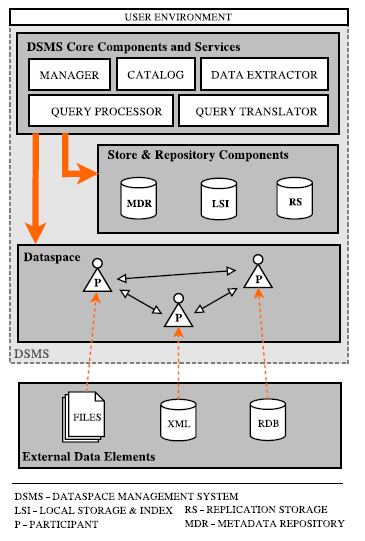
\includegraphics[width=0.75\textwidth]{figures/TowardsRealizationOfDataspaces2.png}
	\end{center}
	\caption{System architecture}
	\label{TowardsRealizationOfDataspacesArchitecture}
\end{figure}
Generallly, a Dataspace consists of Dataspace components, the so-called participants, and relationships between the participants. Components are individual data sources, such as relational databases, text databases, XML databases, data stream systems, web services or other data archives.\\
A Dataspace component includes a description for describing what data it contains, which storage formats are used and which query mechanisms are supported. In addition it contains information about the storage location of the data and whether the data was replicated, equally it contains information about relationships to other participants. The information and data are marked if they are added by the management system, the user or were automatically generated.  \\
Each participant is described the same way as the components and is subsequently registered within the catalog. Thus they are available as data sources for a more abstracted layer, which provides global query and search methods. This global layer is embedded in the DMS. It supports the user to create new Dataspace components, to add relationships between other participants, to register participants within the catalog, to browse the catalog for available participants, to decide whether to share all or only  selected participants within a community including assignments of rights, and to search all or only selected participants of a Dataspace.\\
As each participants is managed by its own and thus is responsible for its data management such as data update, recovery and replica, it isn't a task of the DMS to change the data represented by the participants. Therefore, the DMS has no administration privileges for writing and changing content of the data of a participant. But the DMS provides possibilities to add missing data management services, such as data replication, transformation, download, upload, etc.. 

\textbf{Managing Sub-Dataspaces}\\
The idea behind a Sub-Dataspace is to create a new Dataspace that is included by a another and thus is a subset of a  bigger Dataspace. This functionality is needed for access privileges and security management. An administrator of a Dataspace is thus able to define different data access rights for certain groups.  
